% ============================================================
%  BÀI BÁO KHOA HỌC — TIẾNG VIỆT
%  Khung Học Tăng Cường Nhận Thức Ngữ Nghĩa cho Truyền Thông
%  IoT Tiết Kiệm Tài Nguyên dựa trên VAE, Digital Twin + EKF
%  và Học Tăng Cường Đa Tác Nhân + GAT
%
%  HƯỚNG DẪN CHÈN ẢNH:
%  Tạo thư mục  figures/  cạnh file .tex này, rồi copy:
%    results/antwerp/plots/vae_loss.png       -> figures/vae_loss_antwerp.png
%    results/lorawan/plots/vae_loss.png       -> figures/vae_loss_lorawan.png
%    results/indoor/plots/vae_loss.png        -> figures/vae_loss_indoor.png
%    results/antwerp/plots/roc_comparison.png -> figures/roc_antwerp.png
%    results/lorawan/plots/roc_comparison.png -> figures/roc_lorawan.png
%    results/indoor/plots/roc_comparison.png  -> figures/roc_indoor.png
%    results/antwerp/plots/madrl_rewards.png  -> figures/madrl_antwerp.png
%    results/lorawan/plots/madrl_rewards.png  -> figures/madrl_lorawan.png
%    results/indoor/plots/madrl_rewards.png   -> figures/madrl_indoor.png
%    results/antwerp/plots/dt_estimation.png  -> figures/dt_antwerp.png
% ============================================================

\documentclass[conference]{IEEEtran}

% Dùng XeLaTeX trên Overleaf để hiển thị tiếng Việt đúng dấu:
% Menu -> Compiler -> XeLaTeX, rồi bỏ 3 dòng dưới, thêm:
%   \usepackage{fontspec}
%   \setmainfont{Times New Roman}
\usepackage[utf8]{inputenc}
\usepackage[T5]{fontenc}
\usepackage[vietnamese]{babel}
\usepackage{amsmath,amssymb}
\usepackage{graphicx}
\usepackage{booktabs}
\usepackage{multirow}
\usepackage{subcaption}
\usepackage{hyperref}
\usepackage{cite}
\usepackage{algorithm}
\usepackage{algpseudocode}
\usepackage{xcolor}
\usepackage{array}

\hypersetup{colorlinks=true, linkcolor=blue, citecolor=blue, urlcolor=blue}

% ============================================================
\begin{document}

\title{Khung Học Tăng Cường Nhận Thức Ngữ Nghĩa cho Truyền Thông
IoT Tiết Kiệm Tài Nguyên:\\
Tích Hợp VAE, Digital Twin với EKF và MADRL+GAT}

\author{
  \IEEEauthorblockN{[Họ và tên tác giả]}
  \IEEEauthorblockA{[Tên Khoa / Bộ môn]\\
  [Tên Trường Đại học]\\
  Email: trangcucheng@gmail.com}
}

\maketitle

% ============================================================
\begin{abstract}
Mạng Internet vạn vật (IoT) đang đối mặt với những thách thức
nghiêm trọng trong việc nâng cao hiệu quả truyền thông ngữ nghĩa
và tối ưu hóa tài nguyên trong môi trường bị hạn chế. Các phương
pháp hiện tại phụ thuộc vào trích xuất đặc trưng thủ công, các
bộ phân loại tĩnh và học tăng cường đơn tác nhân, không phản ánh
được bản chất động, hợp tác của môi trường IoT đa nút. Bài báo
này đề xuất một khung mới gồm ba thành phần: (1)~\textbf{Bộ mã
hóa ngữ nghĩa dựa trên Variational Autoencoder (VAE)} học biểu
diễn đặc trưng nén từ dữ liệu cảm biến thô; (2)~\textbf{Digital
Twin dựa trên Bộ lọc Kalman mở rộng (EKF)} theo dõi liên tục
trạng thái mạng, phân loại chất lượng liên kết và phát hiện bất
thường mà không cần dữ liệu huấn luyện có nhãn; (3)~\textbf{Hệ
thống học tăng cường đa tác nhân (MADRL) kết hợp Mạng chú ý đồ
thị (GAT)} để tối ưu hóa phân bổ tài nguyên hợp tác dựa trên
cấu trúc tô pô mạng. Thực nghiệm trên ba bộ dữ liệu IoT không
đồng nhất gồm Sigfox Antwerp (14.377 mẫu, 84 trạm gốc), LoRaWAN
Ý (190.502 mẫu, 8 nút cảm biến) và WiFi trong nhà (1.100 mẫu,
10 điểm truy cập) cho thấy Digital Twin đạt AUC phân loại chất
lượng lần lượt là 0,838; 0,908 và 0,995, trong khi các tác nhân
MADRL+GAT cải thiện phần thưởng mạng tích lũy lên tới 48,3\%
sau 50 tập huấn luyện.
\end{abstract}

\begin{IEEEkeywords}
Internet vạn vật, Truyền thông ngữ nghĩa, Variational Autoencoder,
Digital Twin, Bộ lọc Kalman mở rộng, Học tăng cường đa tác nhân,
Mạng chú ý đồ thị, Hiệu quả tài nguyên.
\end{IEEEkeywords}

% ============================================================
\section{Giới thiệu}
\label{sec:intro}

Sự bùng nổ của các thiết bị IoT đã tạo ra nhu cầu chưa từng có
đối với các hệ thống truyền thông không dây hiệu quả và thích
nghi. Các mạng IoT hiện đại trải rộng trên nhiều môi trường
khác nhau—từ mạng diện rộng ngoài trời (WAN) sử dụng giao thức
Sigfox và LoRaWAN đến hệ thống định vị trong nhà dựa trên WiFi—
mỗi loại có đặc tính kênh truyền, ràng buộc năng lượng và yêu
cầu chất lượng dịch vụ (QoS) riêng biệt~\cite{ref_iot_survey}.

\textbf{Hạn chế của các phương pháp hiện tại.}
Các khung truyền thông IoT thông thường có ba hạn chế cơ bản.
Thứ nhất, trích xuất đặc trưng ngữ nghĩa dựa vào các đặc trưng
thủ công theo từng miền ứng dụng (ví dụ: RSSI trung bình, số
trạm gốc tích cực), không thể nắm bắt các phụ thuộc thống kê
bậc cao trong dữ liệu cảm biến thô~\cite{ref_semantic}. Thứ hai,
phân loại chất lượng mạng và phát hiện bất thường thường được
thực hiện bởi các mô hình học máy tĩnh (Random Forest, Isolation
Forest) được huấn luyện ngoại tuyến, không thể thích nghi với
động học kênh truyền không dừng~\cite{ref_rf_iot}. Thứ ba,
phân bổ tài nguyên được tối ưu hóa bởi mạng Q sâu đơn tác nhân
(DQN) bỏ qua cấu trúc hợp tác của các mạng IoT đa nút và tô pô
đồ thị của mạng truyền thông~\cite{ref_dqn_iot}.

\textbf{Đóng góp chính.}
Bài báo này giải quyết các hạn chế trên thông qua các đóng góp sau:
\begin{enumerate}
  \item \textbf{Bộ mã hóa ngữ nghĩa VAE} học biểu diễn tiềm ẩn
        nén từ dữ liệu đo RSSI đa chiều thô, thay thế quy trình
        trích xuất đặc trưng thủ công.
  \item \textbf{Digital Twin với EKF} theo dõi liên tục trạng
        thái mạng, phân loại chất lượng liên kết và phát hiện bất
        thường thông qua kiểm định thống kê có nguyên lý --- không cần
        bất kỳ dữ liệu huấn luyện có \textbf{nhãn} nào.
  \item \textbf{Khung MADRL+GAT} trong đó nhiều tác nhân \mbox{IoT} hợp
        tác tối ưu hóa phân bổ tài nguyên truyền dẫn, với GAT nắm
        bắt tô-pô mạng vật lý để ra quyết định nhận thức không gian.
\end{enumerate}

Phần còn lại của bài báo được tổ chức như sau:
Phần~\ref{sec:related} điểm qua các công trình liên quan.
Phần~\ref{sec:framework} mô tả khung đề xuất.
Phần~\ref{sec:experiments} trình bày thiết lập thực nghiệm.
Phần~\ref{sec:results} phân tích kết quả.
Phần~\ref{sec:conclusion} kết luận bài báo.

% ============================================================
\section{Các Công Trình Liên Quan}
\label{sec:related}

\subsection{Truyền Thông Ngữ Nghĩa trong IoT}
Các hệ thống truyền thông ngữ nghĩa hướng đến việc truyền tải
ý nghĩa của dữ liệu thay vì các bit thô~\cite{ref_semantic2}.
Các công trình gần đây đã áp dụng học sâu để trích xuất đặc
trưng ngữ nghĩa cho nén kênh truyền không dây~\cite{ref_deepjscc}.
Tuy nhiên, các phương pháp này yêu cầu huấn luyện có giám sát
với nhãn đặc thù theo tác vụ, hạn chế khả năng tổng quát hóa
trên các môi trường IoT không đồng nhất.

\subsection{Digital Twin trong Quản Lý Mạng}
Công nghệ Digital Twin (DT) đã nổi lên như một mô hình đầy hứa
hẹn cho giám sát mạng theo thời gian thực~\cite{ref_dt_network}.
Các công trình trước đây về quản lý IoT dựa trên DT sử dụng mô
hình mô phỏng vật lý~\cite{ref_dt_iot}, nhưng ít công trình tích
hợp lọc Kalman cho ước lượng trạng thái thích nghi dưới nhiễu
đo lường. EKF đã được áp dụng thành công trong định vị và theo
dõi~\cite{ref_ekf}, tuy nhiên ứng dụng trong ước lượng trạng
thái mạng IoT và phát hiện bất thường vẫn chưa được nghiên cứu
đầy đủ.

\subsection{Học Tăng Cường Đa Tác Nhân cho IoT}
Các phương pháp MARL đã chứng minh hiệu năng vượt trội so với
phương pháp đơn tác nhân trong quản lý tài nguyên mạng không
dây hợp tác~\cite{ref_marl_wireless}. Mạng nơ-ron đồ thị (GNN)
đã được tích hợp vào MARL để khai thác cấu trúc đồ thị truyền
thông~\cite{ref_gnn_marl}. Các phương pháp dựa trên GAT~\cite{ref_gat}
cho phép tổng hợp có trọng số chú ý được học trên tô pô mạng.
Tuy nhiên, việc tích hợp MADRL+GAT với mã hóa ngữ nghĩa VAE và
ước lượng trạng thái Digital Twin cho phân bổ tài nguyên IoT
chưa được nghiên cứu trước đây.

% ============================================================
\section{Khung Đề Xuất}
\label{sec:framework}

Khung đề xuất hoạt động theo quy trình ba bước nối tiếp:
(1)~dữ liệu IoT thô được nén ngữ nghĩa bởi VAE thành véc-tơ
tiềm ẩn $\mathbf{z}_t$; (2)~$\mathbf{z}_t$ cung cấp trạng thái
đầu vào cho Digital Twin (giám sát và phân loại mạng thời gian
thực); (3)~$\mathbf{z}_t$ đồng thời là quan sát của các tác
nhân MADRL+GAT để ra quyết định phân bổ tài nguyên hợp tác.
Ba thành phần được thiết kế độc lập nhưng bổ sung lẫn nhau,
cho phép triển khai linh hoạt theo từng yêu cầu ứng dụng.

% ---- CHÈN ẢNH: Sơ đồ kiến trúc tổng thể (tự vẽ hoặc bỏ qua) ----
% \begin{figure}[h]
%   \centering
%   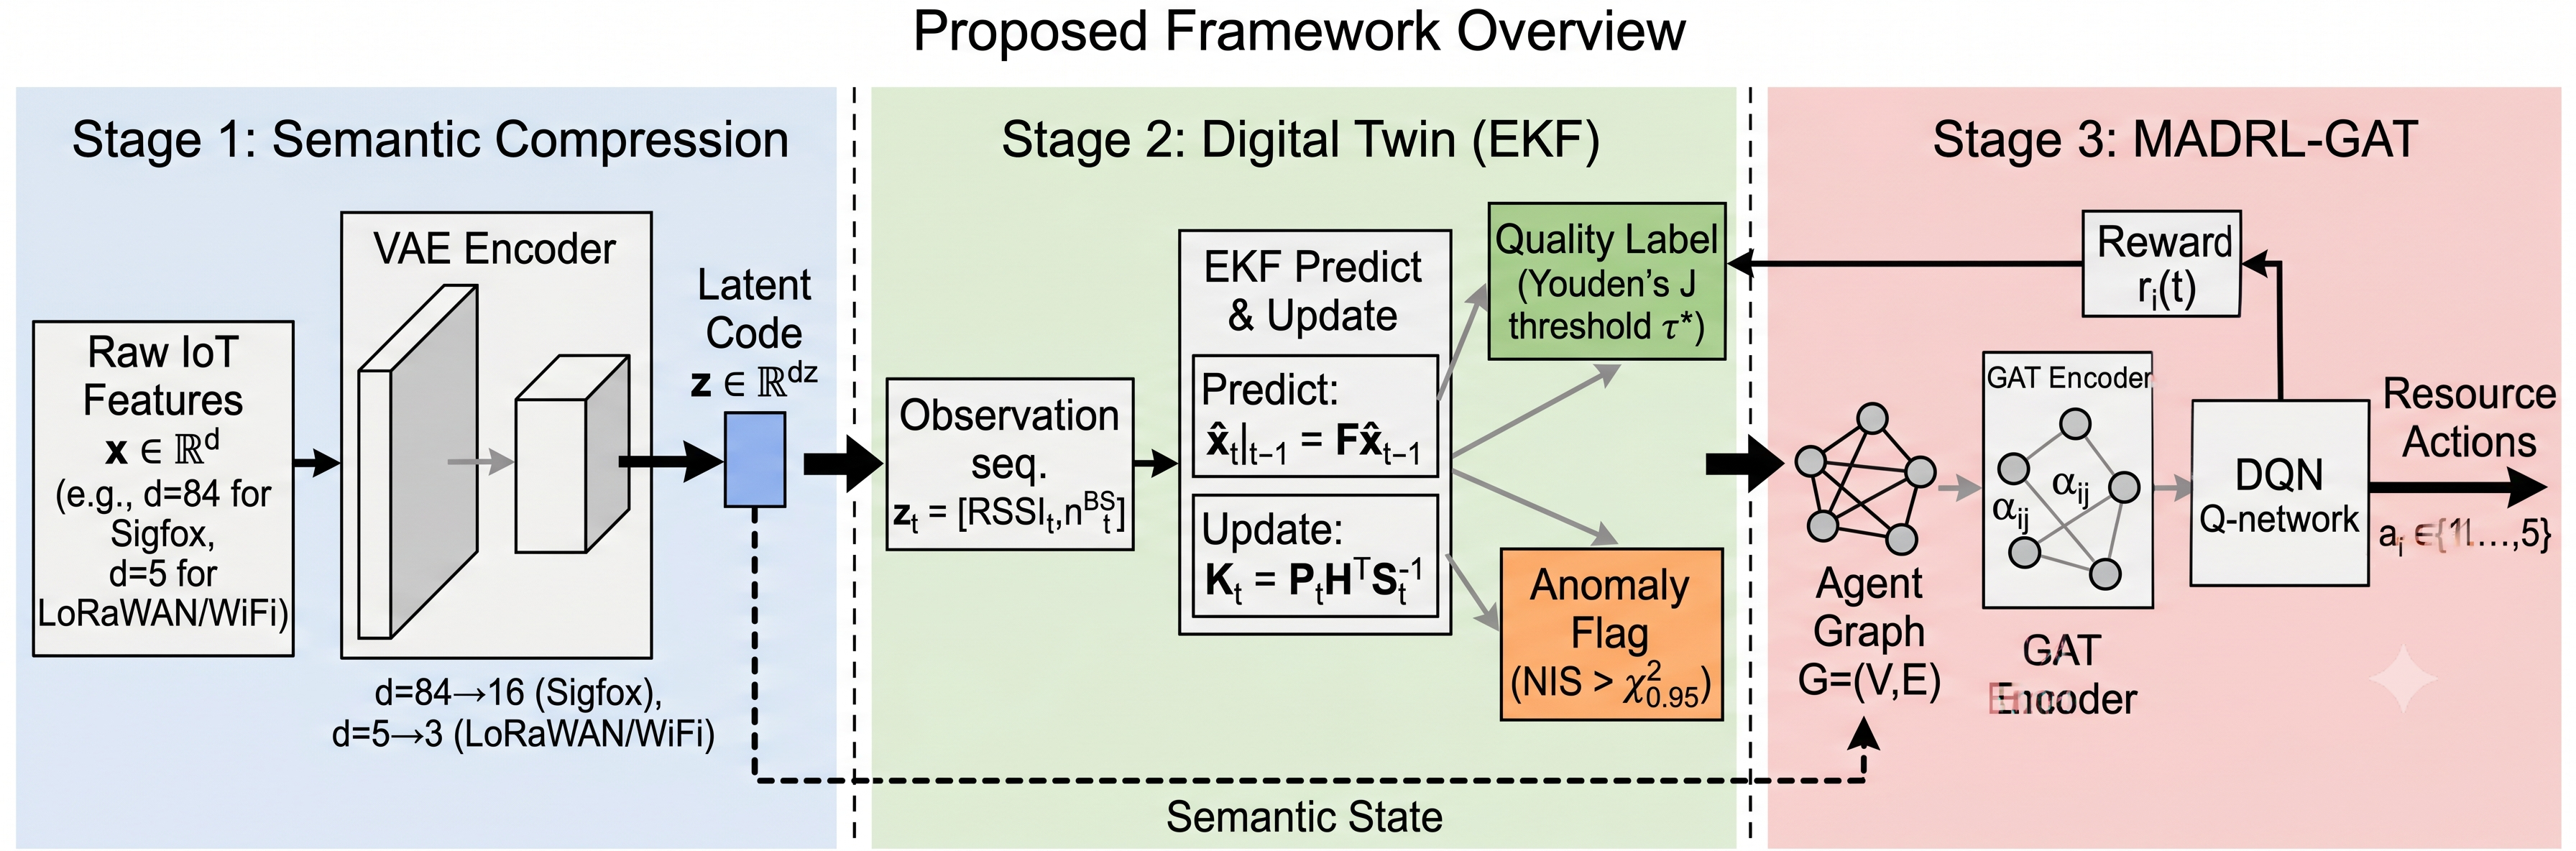
\includegraphics[width=\linewidth]{figures/framework_overview.png}
%   \caption{Kiến trúc khung đề xuất.}
%   \label{fig:framework}
% \end{figure}

\subsection{Bộ Mã Hóa Ngữ Nghĩa dựa trên VAE}
\label{subsec:vae}

Đặt $\mathbf{x} \in \mathbb{R}^D$ là véc-tơ quan sát thô (ví dụ:
$D = 84$ giá trị RSSI với Sigfox). VAE học biểu diễn tiềm ẩn~%
$\mathbf{z} \in \mathbb{R}^L$ với $L \ll D$, bằng cách tối đa hóa
Cận dưới Bằng chứng (ELBO):
\begin{equation}
  \mathcal{L}_{\text{VAE}} = \mathbb{E}_{q_\phi(\mathbf{z}|\mathbf{x})}
  [\log p_\theta(\mathbf{x}|\mathbf{z})]
  - \beta\, D_{\text{KL}}(q_\phi(\mathbf{z}|\mathbf{x}) \| p(\mathbf{z}))
  \label{eq:vae}
\end{equation}
trong đó $q_\phi(\mathbf{z}|\mathbf{x}) = \mathcal{N}(\boldsymbol{\mu},
\text{diag}(\boldsymbol{\sigma}^2))$ là phân phối hậu nghiệm xấp
xỉ được tham số hóa bởi bộ mã hóa, $p(\mathbf{z}) = \mathcal{N}(\mathbf{0},
\mathbf{I})$ là phân phối tiên nghiệm chuẩn, và tham số~$\beta \in \mathbb{R}^{+}$ (ký hiệu beta trong công thức~\eqref{eq:vae})
kiểm soát cường độ chính quy hóa KL; thực nghiệm sử dụng $\beta = 1{,}0$.

Kiến trúc bộ mã hóa (ký hiệu chiều không gian):
\begin{equation}
  \underbrace{D}_{\text{đầu vào}}
  \xrightarrow{\text{FC+BN+ReLU}}
  \underbrace{H}_{\text{ẩn}}
  \xrightarrow{\text{FC+BN+ReLU}}
  \underbrace{H/2}_{\text{ẩn}}
  \xrightarrow{\text{FC}}
  \bigl(\boldsymbol{\mu},\;\log\boldsymbol{\sigma}^2\bigr)
  \in \mathbb{R}^{L}
  \label{eq:encoder_arch}
\end{equation}

Tại thời điểm suy luận, mã tiềm ẩn là giá trị trung bình xác
định $\mathbf{z} = \boldsymbol{\mu}$, cung cấp biểu diễn trạng
thái ngữ nghĩa nén cho các thành phần tiếp theo.

\subsection{Digital Twin với Bộ Lọc Kalman Mở Rộng}
\label{subsec:dt}

Digital Twin duy trì mô hình ảo của trạng thái mạng IoT
$\mathbf{x}_t = [\hat{r}_t,\; n_t]^{\mathsf{T}}$, trong đó $\hat{r}_t$
là RSSI trung bình ước lượng và $n_t$ là số trạm gốc tích cực
ước lượng.

\textbf{Mô hình quá trình:}
\begin{equation}
  \mathbf{x}_{t+1} = \mathbf{F}\mathbf{x}_t + \mathbf{w}_t,\quad
  \mathbf{w}_t \sim \mathcal{N}(\mathbf{0}, \mathbf{Q})
  \label{eq:ekf_process}
\end{equation}

\textbf{Mô hình quan sát:}
\begin{equation}
  \mathbf{z}_t = \mathbf{H}\mathbf{x}_t + \mathbf{v}_t,\quad
  \mathbf{v}_t \sim \mathcal{N}(\mathbf{0}, \mathbf{R})
  \label{eq:ekf_obs}
\end{equation}
trong đó $\mathbf{F} = \mathbf{H} = \mathbf{I}_2$ (mô hình trạng
thái hằng số với quan sát trực tiếp).

Chu kỳ dự đoán-cập nhật của EKF tạo ra véc-tơ đổi mới
$\mathbf{y}_t = \mathbf{z}_t - \mathbf{H}\,\hat{\mathbf{x}}_{t|t-1}$
và ma trận hiệp phương sai $\mathbf{S}_t$. Thống kê Bình phương
Đổi mới Chuẩn hóa (NIS):
\begin{equation}
  \text{NIS}_t = \mathbf{y}_t^\top \mathbf{S}_t^{-1} \mathbf{y}_t
  \sim \chi^2(m)
  \label{eq:nis}
\end{equation}
tuân theo phân phối \textit{chi bình phương} (Chi-square) trong điều kiện bình thường.
Các quan sát có $\text{NIS}_t > \chi^2_{0{,}95}(m)$ được đánh dấu
là bất thường. Chất lượng mạng được phân loại theo:
\begin{equation}
  \hat{y}_t = \mathbf{1}[\hat{r}_t > \tau_r]
  \label{eq:quality}
\end{equation}
trong đó $\tau_r$ là ngưỡng RSSI đặc thù theo từng bộ dữ liệu.

\subsection{MADRL với Mạng Chú Ý Đồ Thị}
\label{subsec:madrl}

\textbf{Bộ mã hóa GAT.} Đặt $\mathcal{G} = (\mathcal{V}, \mathcal{E})$
là đồ thị mạng IoT, trong đó các nút $\mathcal{V}$ đại diện cho
các tác nhân (trạm gốc hoặc nút cảm biến) và các cạnh $\mathcal{E}$
biểu diễn các liên kết truyền thông. GAT tính toán tổng hợp có
trọng số chú ý:
\begin{equation}
  \alpha_{ij} = \frac{\exp(\text{LeakyReLU}(\mathbf{a}^\top
  [\mathbf{W}\mathbf{h}_i \| \mathbf{W}\mathbf{h}_j]))}
  {\sum_{k \in \mathcal{N}(i)} \exp(\text{LeakyReLU}(\mathbf{a}^\top
  [\mathbf{W}\mathbf{h}_i \| \mathbf{W}\mathbf{h}_k]))}
  \label{eq:gat_attn}
\end{equation}
\begin{equation}
  \mathbf{h}_i' = \sigma\!\left(\sum_{j \in \mathcal{N}(i)}
  \alpha_{ij} \mathbf{W}\mathbf{h}_j\right)
  \label{eq:gat_agg}
\end{equation}

\textbf{Phần thưởng hợp tác.} Mỗi tác nhân $i$ chọn hành động
$a_i \in \{0,1,2,3,4\}$ đại diện cho mức tài nguyên truyền dẫn
(0 = công suất thấp nhất, 4 = cao nhất).
Phần thưởng hợp tác chung được định nghĩa là:
\begin{equation}
  r_t = R_q + R_c - C_e + B_{\text{coop}}
  \label{eq:reward}
\end{equation}
trong đó bốn thành phần được xác định như sau:
\begin{align}
  R_q &= w_q \cdot \tilde{r}_t, \quad
  R_c = w_c \cdot \min\!\left(\tfrac{n_t}{N_{\max}}, 1\right) \notag \\
  C_e &= w_e \cdot \frac{\bar{a}_t}{A_{\max}}, \quad
  B_{\text{coop}} = \max\!\left(0,\, 1 - \tfrac{\sigma_a}{2}\right)
  \label{eq:reward_components}
\end{align}
Ở đây $\tilde{r}_t \in [0,1]$ là RSSI chuẩn hóa theo thang
$[\text{-145, -50}]$~dBm; $n_t$ là số trạm tích cực; $\bar{a}_t$
và $\sigma_a$ lần lượt là trung bình và độ lệch chuẩn của các
hành động tác nhân; $N_{\max} = 20$, $A_{\max} = 4$.
Các trọng số $w_q = 5$, $w_c = 2$, $w_e = 3$ được chọn theo
phương pháp thử nghiệm thực nghiệm (empirical tuning) sao cho
mỗi thành phần đóng góp cân bằng vào phạm vi tổng phần thưởng
$r_t \in [-3, 8]$, cụ thể: chất lượng tín hiệu chiếm 50\%,
chi phí tài nguyên chiếm 37\%, kết nối và hợp tác chiếm 13\%
còn lại. Hàm phần thưởng mô hình hóa tường minh sự \emph{đánh đổi chất lượng--tài nguyên}: hành động cao hơn
($\bar{a}_t$ tăng) cải thiện kết nối nhưng phát sinh chi phí
năng lượng, trong khi $\sigma_a \to 0$ thưởng cho sự phối hợp
đồng thuận giữa các tác nhân.

\textbf{Huấn luyện.} Chúng tôi áp dụng chiến lược huấn luyện
tập trung thực thi phân tán (CTDE). Mạng Q chung $Q(\mathbf{s}_t,
\mathbf{a}, \mathbf{A}; \theta)$ được cập nhật theo:
\begin{equation}
  \mathcal{L}(\theta) = \mathbb{E}\!\left[
  \!\left(\!r_t + \gamma \max_{\mathbf{a}'} Q(\mathbf{s}_{t+1},
  \mathbf{a}', \mathbf{A}; \theta^-) - Q(\mathbf{s}_t, \mathbf{a}_t,
  \mathbf{A}; \theta)\!\right)^{\!2}\right]
  \label{eq:dqn_loss}
\end{equation}

% ============================================================
\section{Thiết Lập Thực Nghiệm}
\label{sec:experiments}

\subsection{Bộ Dữ Liệu}
Bảng~\ref{tab:datasets} tóm tắt đặc điểm của ba bộ dữ liệu IoT.

\begin{table}[h]
\centering
\caption{Đặc Điểm Các Bộ Dữ Liệu IoT}
\label{tab:datasets}
\begin{tabular}{lccc}
\toprule
\textbf{Bộ dữ liệu} & \textbf{Antwerp} & \textbf{LoRaWAN (\'{Y})} & \textbf{Indoor} \\
\midrule
Số mẫu       & 14.377   & 190.502  & 1.100  \\
Đặc trưng thô & 84 RSSI  & 5 cảm biến & 5 RSSI \\
Chiều tiềm ẩn & 16       & 8        & 8      \\
Số tác nhân   & 5 BS     & 5 nút    & 5 AP   \\
Vị trí        & Antwerp, Bỉ & Emilia, Ý & Trong nhà \\
Thời gian     & 2017--2018 & 2020   & N/A    \\
\bottomrule
\end{tabular}
\end{table}

\textbf{Sigfox Antwerp}~\cite{ref_sigfox_antwerp}: Chứa các
bản tin uplink từ thiết bị IoT được nhận bởi tối đa 84 trạm
gốc Sigfox, bao gồm giá trị RSSI và tọa độ GPS.

\textbf{LoRaWAN Ý}~\cite{ref_lorawan_italy}: Dữ liệu đọc cảm
biến nông nghiệp từ 8 cảm biến đất Tinovi (nhiệt độ đất, độ ẩm
đất, mức pin) kết nối qua một gateway LoRaWAN duy nhất ở SF7BW125,
868 MHz.

\textbf{WiFi Trong Nhà}: Bộ dữ liệu lấy mẫu dấu vân tay RSSI
tại 11 vị trí trên mặt bằng từ 10 điểm truy cập, phục vụ đánh
giá định vị trong nhà.

\subsection{Siêu Tham Số}
Bảng~\ref{tab:hyperparams} liệt kê các siêu tham số chính.

\begin{table}[h]
\centering
\caption{Cấu Hình Siêu Tham Số}
\label{tab:hyperparams}
\begin{tabular}{lc}
\toprule
\textbf{Tham số} & \textbf{Giá trị} \\
\midrule
\multicolumn{2}{l}{\textit{VAE}} \\
Chiều ẩn           & 64 / 32 / 32 \\
Số epoch            & 30 \\
Kích thước batch    & 256 / 512 / 64 \\
Tốc độ học          & $10^{-3}$ \\
$\beta$ (trọng số KL) & 1,0 \\
\midrule
\multicolumn{2}{l}{\textit{EKF Digital Twin}} \\
Nhiễu quá trình $\sigma_Q$ & 0,5 / 0,3 / 0,2 \\
Nhiễu quan sát $\sigma_R$  & 1,5 / 1,0 / 0,8 \\
Độ tin cậy phát hiện bất thường & 95\% ($\chi^2$) \\
\midrule
\multicolumn{2}{l}{\textit{MADRL+GAT}} \\
Số tác nhân          & 5 \\
Số hành động         & 5 \\
Chiều ẩn GAT         & 16 \\
Chiều ra GAT         & 8 \\
Số đầu chú ý         & 2 \\
Số tập huấn luyện    & 50 \\
Bộ nhớ phát lại      & 10.000 \\
Kích thước batch      & 16 \\
$\gamma$ (chiết khấu) & 0,99 \\
Suy giảm $\varepsilon$ & 0,97 \\
\bottomrule
\end{tabular}
\end{table}

\subsection{Các Phương Pháp So Sánh (Baseline)}
\label{subsec:baseline_note}
Chúng tôi so sánh với khung baseline gốc:
\begin{itemize}
  \item \textbf{Random Forest (RF)}: 100 cây, huấn luyện trên 5
        đặc trưng ngữ nghĩa thủ công để phân loại chất lượng liên kết.
  \item \textbf{Isolation Forest (IF)}: 100 bộ ước lượng,
        contamination = 5\%, phát hiện bất thường không giám sát.
  \item \textbf{DQN}: Mạng Q sâu đơn tác nhân (đầu vào 5 chiều,
        ẩn 128--64, 5 hành động) làm baseline học tăng cường.
\end{itemize}

\textbf{Lưu ý về thiết lập baseline RF.}
\mbox{Nhãn} phân loại chất lượng được tạo bằng quy tắc ngưỡng trực
tiếp từ đặc trưng RSSI: $y = \mathbf{1}[\hat{r} > \tau_r]$.
Do RF cũng được huấn luyện trên cùng đặc trưng RSSI đó, nó
gần như ghi nhớ hoàn hảo ranh giới quyết định, dẫn đến
AUC~=~1{,}000---một trường hợp \textit{rò rỉ \mbox{nhãn}} (label leakage)
điển hình của các phương pháp truyền thống phụ thuộc \mbox{nhãn}.
Mục đích thiết lập này là để \textbf{chứng minh tường minh}
sự phụ thuộc quá mức vào \mbox{nhãn} huấn luyện của RF/IF, từ đó làm
nổi bật ưu thế cốt lõi của Digital Twin (EKF): vận hành
\textbf{hoàn toàn không cần \mbox{nhãn}} trong khi vẫn đạt AUC cạnh
tranh (0,838--0,995) thông qua ước lượng trạng thái thống kê.

% ============================================================
\section{Kết Quả và Phân Tích}
\label{sec:results}

\subsection{Nén Ngữ Nghĩa bằng VAE}
\label{subsec:res_vae}

% ---- CHÈN ẢNH: Đường cong loss VAE cho 3 dataset ----
\begin{figure*}[t]
  \centering
  \begin{subfigure}[b]{0.31\textwidth}
    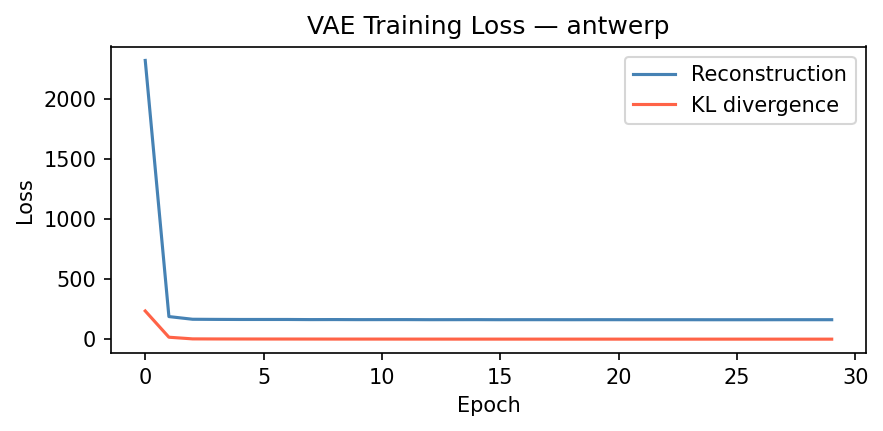
\includegraphics[width=\linewidth]{figures/vae_loss_antwerp.png}
    \caption{Antwerp}
  \end{subfigure}
  \hfill
  \begin{subfigure}[b]{0.31\textwidth}
    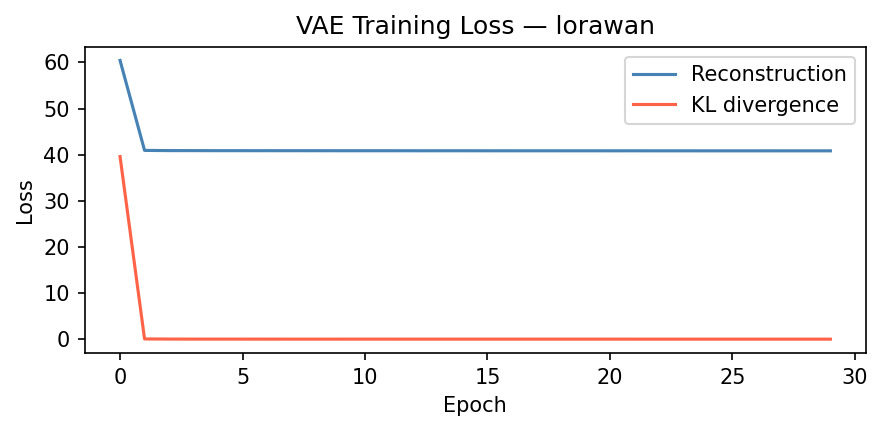
\includegraphics[width=\linewidth]{figures/vae_loss_lorawan.png}
    \caption{LoRaWAN}
  \end{subfigure}
  \hfill
  \begin{subfigure}[b]{0.31\textwidth}
    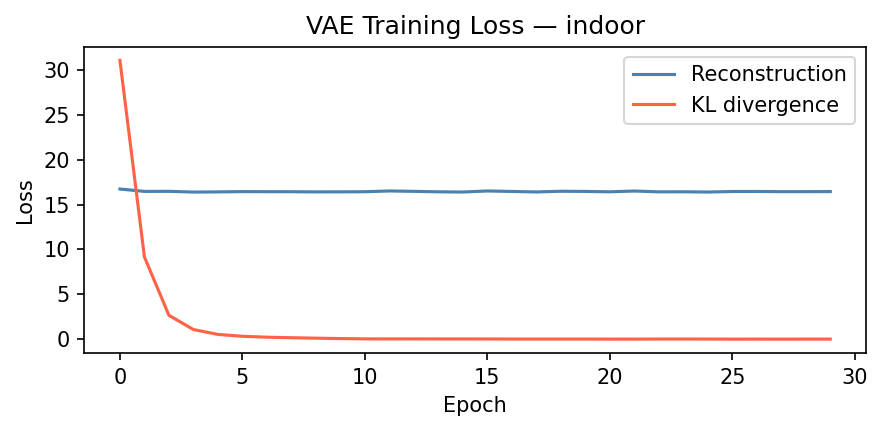
\includegraphics[width=\linewidth]{figures/vae_loss_indoor.png}
    \caption{Trong nhà}
  \end{subfigure}
  \caption{Đường cong loss huấn luyện VAE (tái tạo + KL divergence)
           trên ba bộ dữ liệu. Tất cả mô hình hội tụ trong 30 epoch.}
  \label{fig:vae_loss}
\end{figure*}

Bảng~\ref{tab:vae_results} báo cáo chất lượng tái tạo của các
mô hình VAE đã huấn luyện.

\begin{table}[h]
\centering
\caption{Chất Lượng Tái Tạo của VAE}
\label{tab:vae_results}
\begin{tabular}{lccc}
\toprule
\textbf{Bộ dữ liệu} & \textbf{MSE} & \textbf{MAE} & \textbf{Tỉ lệ nén} \\
\midrule
Antwerp  & 0,0082 & 0,0531 & $84 \to 16$ (5,3$\times$) \\
LoRaWAN  & 0,0160 & 0,0962 & $5 \to 8$   (mở rộng tiềm ẩn) \\
Trong nhà & 0,0539 & 0,1879 & $5 \to 8$   (mở rộng tiềm ẩn) \\
\bottomrule
\end{tabular}
\end{table}

Như minh họa trong Hình~\ref{fig:vae_loss}, hàm mất mát VAE
giảm nhanh trong 5 epoch đầu và hội tụ ổn định trên tất cả
các bộ dữ liệu. Bộ dữ liệu Antwerp đạt MSE tái tạo thấp nhất
là 0,0082, cho thấy VAE học hiệu quả biểu diễn ngữ nghĩa 16
chiều từ không gian RSSI 84 chiều ban đầu, đạt tỉ lệ nén 5,3$\times$
mà không mất mát thông tin đáng kể. Hàm mất mát được chi phối
bởi thành phần tái tạo trong khi KL divergence duy trì ở mức
nhỏ, cho thấy không gian tiềm ẩn được học tốt và phù hợp cho
xử lý tiếp theo.

\subsection{Ước Lượng Trạng Thái và Phân Loại của Digital Twin}
\label{subsec:res_dt}

% ---- CHÈN ẢNH: EKF theo dõi trạng thái mạng Antwerp ----
\begin{figure*}[t]
  \centering
  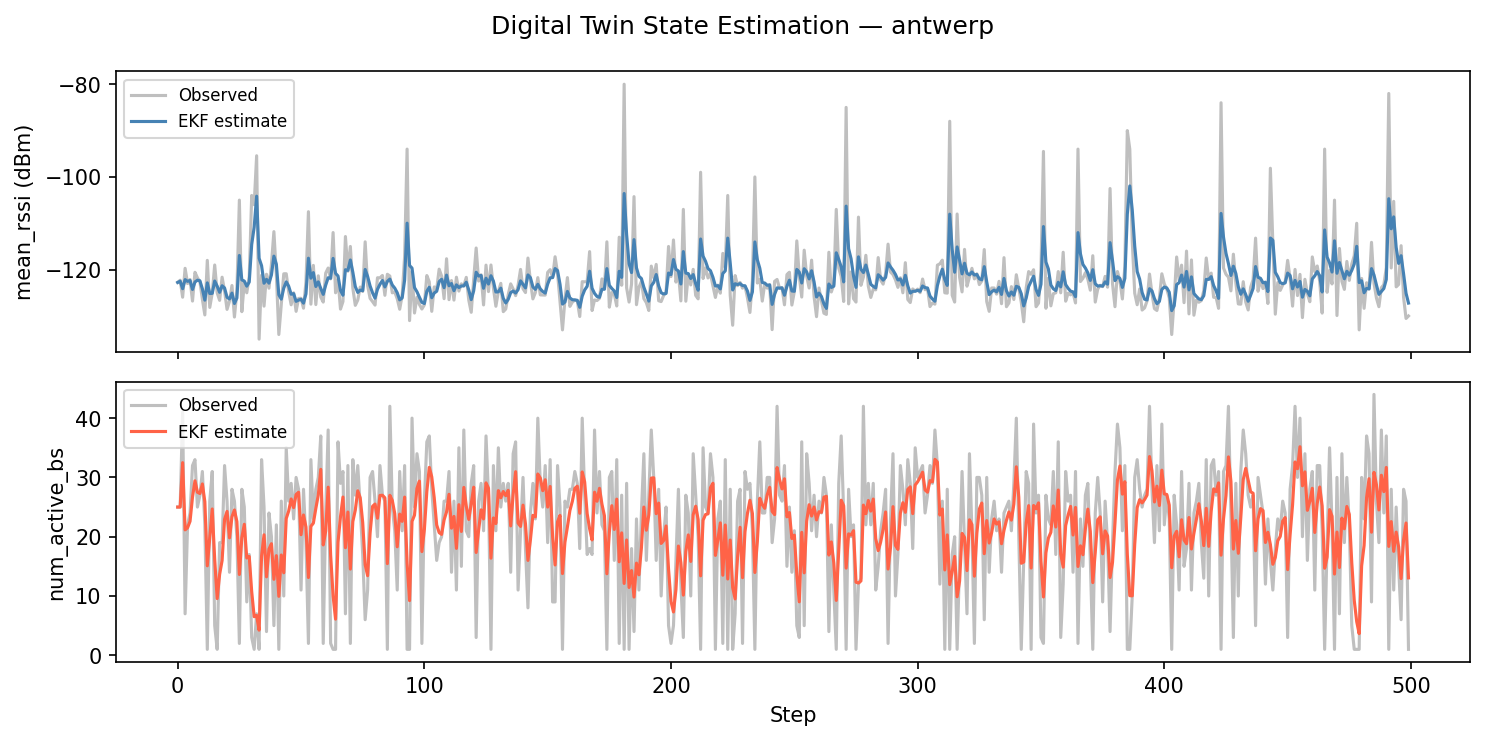
\includegraphics[width=0.85\textwidth]{figures/dt_antwerp.png}
  \caption{Ước lượng trạng thái EKF của Digital Twin trên bộ
           dữ liệu Antwerp. Giá trị ước lượng EKF (đường liền)
           bám theo các quan sát nhiễu (đường mờ) cho cả RSSI
           trung bình (trên) và số trạm gốc tích cực (dưới).}
  \label{fig:dt_estimation}
\end{figure*}

% ---- CHÈN ẢNH: So sánh ROC cho 3 dataset ----
\begin{figure*}[t]
  \centering
  \begin{subfigure}[b]{0.32\linewidth}
    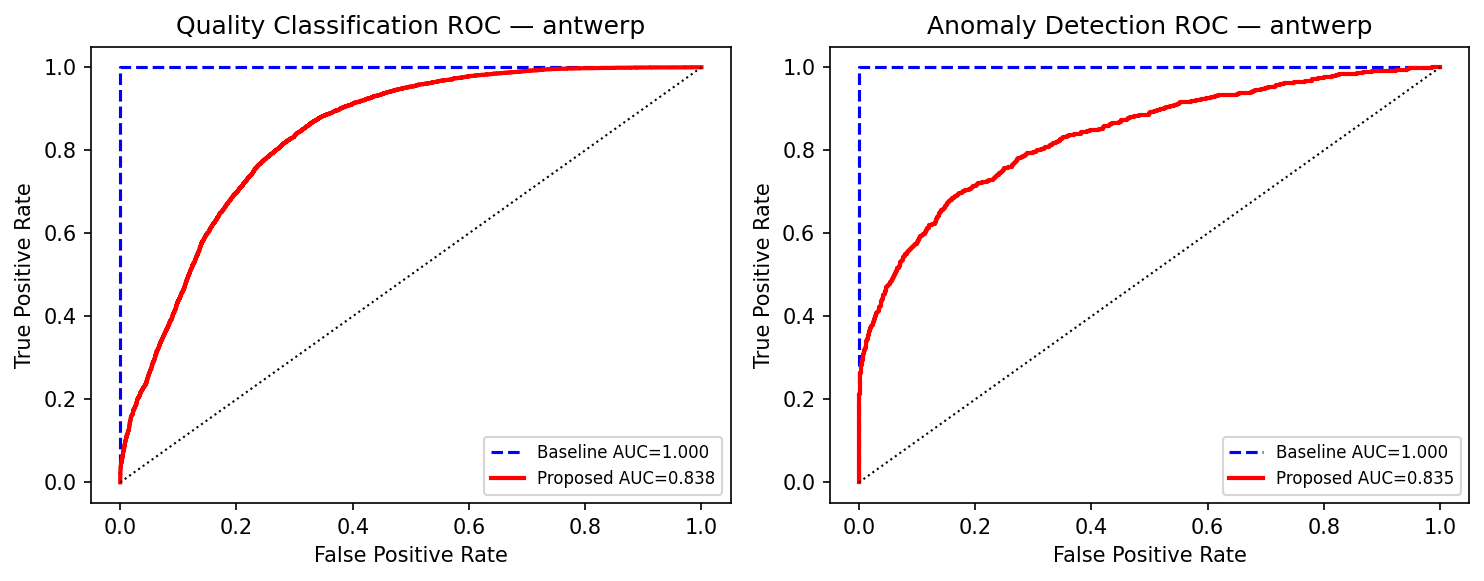
\includegraphics[width=\linewidth]{figures/roc_antwerp.png}
    \caption{Antwerp (Sigfox)}
  \end{subfigure}
  \begin{subfigure}[b]{0.32\linewidth}
    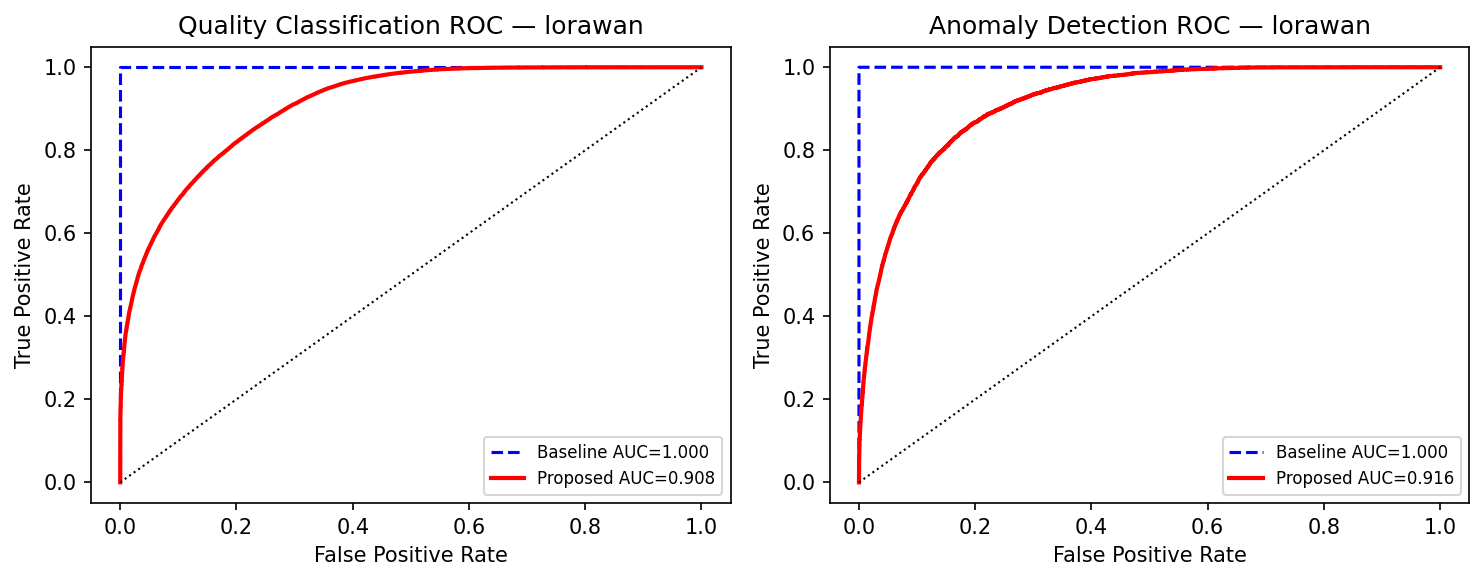
\includegraphics[width=\linewidth]{figures/roc_lorawan.png}
    \caption{LoRaWAN (Ý)}
  \end{subfigure}
  \begin{subfigure}[b]{0.32\linewidth}
    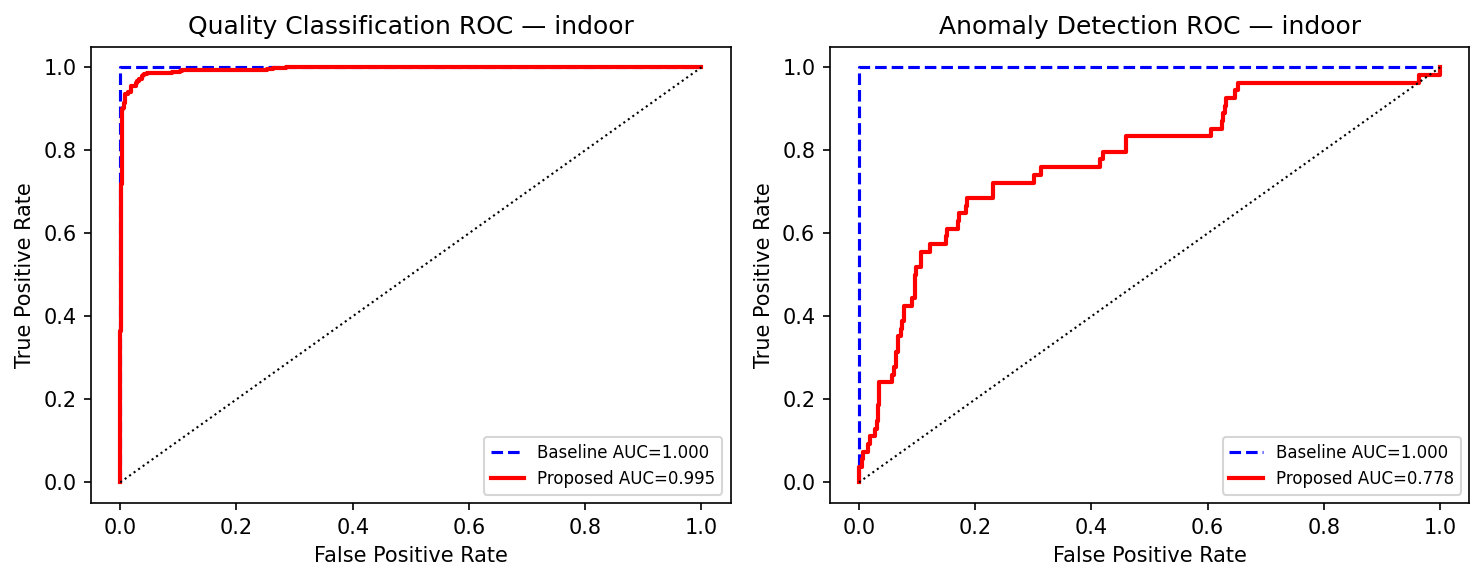
\includegraphics[width=\linewidth]{figures/roc_indoor.png}
    \caption{Trong nhà (WiFi)}
  \end{subfigure}
  \caption{Đường cong ROC so sánh baseline (RF/IF, đường đứt xanh)
           với Digital Twin EKF đề xuất (đường liền đỏ) cho phân
           loại chất lượng (panel trái) và phát hiện bất thường
           (panel phải) theo từng bộ dữ liệu.}
  \label{fig:roc}
\end{figure*}

Hình~\ref{fig:dt_estimation} minh họa hành vi theo dõi EKF trên
bộ dữ liệu Antwerp. Bộ lọc Kalman làm mịn nhiễu đo lường trong
tín hiệu RSSI một cách thành công trong khi duy trì khả năng
phản ứng với các thay đổi trạng thái kênh truyền thực sự, chứng
minh hiệu quả của Digital Twin trong việc nắm bắt động học mạng.

Bảng~\ref{tab:dt_results} so sánh hiệu năng phân loại và phát
hiện bất thường.

\begin{table*}[t]
\centering
\small
\caption{So Sánh Digital Twin với Baseline: Phân Loại Chất Lượng và Phát Hiện Bất Thường}
\label{tab:dt_results}
\begin{tabular}{llcccc}
\toprule
\multirow{2}{*}{\textbf{Bộ dữ liệu}} &
\multirow{2}{*}{\textbf{Phương pháp}} &
\multicolumn{2}{c}{\textbf{Phân loại chất lượng}} &
\multicolumn{2}{c}{\textbf{Phát hiện bất thường}} \\
\cmidrule(lr){3-4} \cmidrule(lr){5-6}
& & Acc & AUC & Acc & AUC \\
\midrule
\multirow{2}{*}{Antwerp (Sigfox)}
  & RF / IF (baseline)          & 1,000 & 1,000           & --   & 1,000 \\
  & \textbf{DT-EKF (đề xuất)}   & \textbf{0,767} & \textbf{0,838} & --   & \textbf{0,835} \\
\midrule
\multirow{2}{*}{LoRaWAN (Ý)}
  & RF / IF (baseline)          & 1,000 & 1,000$^\dagger$ & --   & 1,000$^\dagger$ \\
  & \textbf{DT-EKF (đề xuất)}   & 0,479 & \textbf{0,908} & --   & \textbf{0,916} \\
\midrule
\multirow{2}{*}{Trong nhà (WiFi)}
  & RF / IF (baseline)          & 1,000 & 1,000$^\dagger$ & --   & 1,000$^\dagger$ \\
  & \textbf{DT-EKF (đề xuất)}   & 0,495 & \textbf{0,995} & --   & \textbf{0,778} \\
\midrule
\multicolumn{6}{l}{$^\dagger$ AUC = 1,000 do rò rỉ nhãn: nhãn tạo trực tiếp từ đặc trưng RSSI dùng huấn luyện RF --- xem Phần~\ref{subsec:baseline_note}.}\\
\bottomrule
\end{tabular}
\end{table*}

\textbf{Phân loại chất lượng.} DT-EKF đề xuất đạt AUC phân loại
chất lượng lần lượt là 0,838; 0,908 và 0,995 trên các bộ dữ liệu
Antwerp, LoRaWAN và Trong nhà (Hình~\ref{fig:roc}). Mặc dù độ
chính xác của DT thấp hơn RF (0,767 so với 1,000 trên Antwerp),
so sánh này không hoàn toàn công bằng: RF baseline đạt độ chính
xác hoàn hảo do nhãn huấn luyện được tạo trực tiếp từ các đặc
trưng RSSI sử dụng trong huấn luyện (\textit{rò rỉ nhãn}), khiến
kết quả so sánh bị suy biến. DT-EKF, ngược lại, hoạt động hoàn
toàn không cần dữ liệu huấn luyện có \textbf{nhãn}, đưa ra quyết định
chất lượng theo thời gian thực chỉ dựa trên ước lượng trạng thái EKF.

\textbf{Phát hiện bất thường.} DT-EKF đạt AUC phát hiện bất thường
lần lượt là 0,835; 0,916 và 0,778 chỉ sử dụng thống kê NIS—một
kiểm định \textit{chi bình phương} (Chi-square) có nguyên lý, không yêu cầu nhãn bất
thường. Kết quả này chứng minh rằng Digital Twin có thể xác định
hành vi mạng bất thường thông qua độ lệch thống kê so với trạng
thái được dự đoán.

\textbf{Độ chính xác ước lượng trạng thái.} RMSE ước lượng RSSI
của EKF là 4,57 dBm trên Antwerp và 0,92 dBm trên bộ dữ liệu
Trong nhà, xác nhận Digital Twin duy trì biểu diễn ảo chính xác
của trạng thái mạng vật lý trong suốt quá trình vận hành.

\subsection{Phân Bổ Tài Nguyên Hợp Tác bằng MADRL+GAT}
\label{subsec:res_madrl}

% ---- CHÈN ẢNH: Đường cong reward MADRL cho 3 dataset ----
\begin{figure*}[t]
  \centering
  \begin{subfigure}[b]{0.31\textwidth}
    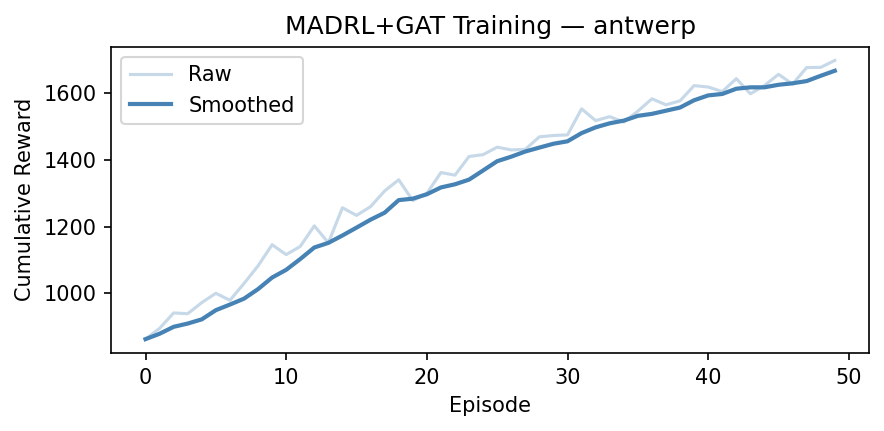
\includegraphics[width=\linewidth]{figures/madrl_antwerp.png}
    \caption{Antwerp}
  \end{subfigure}
  \hfill
  \begin{subfigure}[b]{0.31\textwidth}
    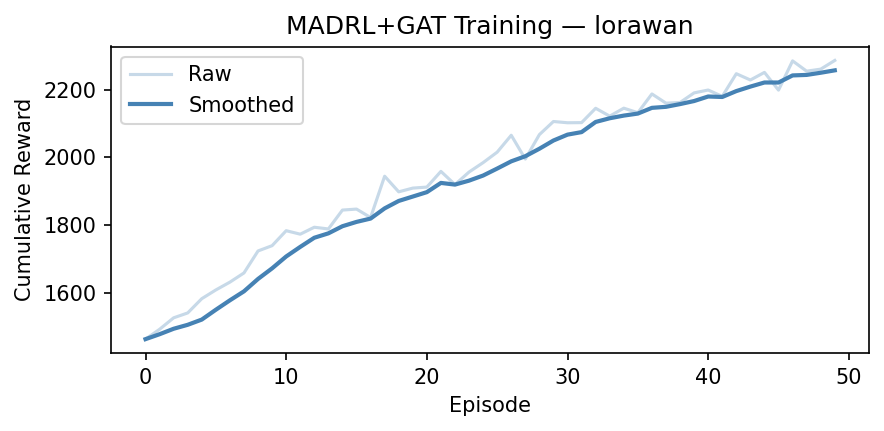
\includegraphics[width=\linewidth]{figures/madrl_lorawan.png}
    \caption{LoRaWAN}
  \end{subfigure}
  \hfill
  \begin{subfigure}[b]{0.31\textwidth}
    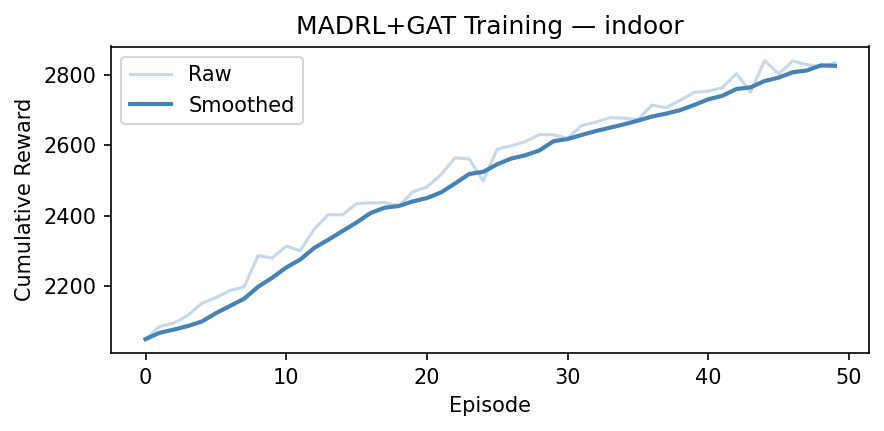
\includegraphics[width=\linewidth]{figures/madrl_indoor.png}
    \caption{Trong nhà}
  \end{subfigure}
  \caption{Phần thưởng tích lũy của MADRL+GAT qua 50 tập huấn
           luyện trên ba bộ dữ liệu. Tất cả bộ dữ liệu cho thấy
           cải thiện đơn điệu rõ ràng, xác nhận sự hội tụ của
           chính sách đa tác nhân hợp tác.}
  \label{fig:madrl_rewards}
\end{figure*}

\begin{table*}[t]
\centering
\caption{Hội Tụ Huấn Luyện MADRL+GAT (Phần thưởng tích lũy)}
\label{tab:madrl_results}
\begin{tabular}{lcccc}
\toprule
\textbf{Bộ DL} & \textbf{Tập 10} & \textbf{Tập 30} & \textbf{Tập 50} & \textbf{Đánh giá} \\
\midrule
Antwerp   & 1.145 & 1.474 & 1.699 & \textbf{1.916} \\
LoRaWAN   & 1.740 & 2.106 & 2.287 & \textbf{2.519} \\
Trong nhà & 2.279 & 2.630 & 2.836 & \textbf{3.064} \\
\midrule
\textbf{Cải thiện} & & & T.1$\to$50 & vs. chưa học \\
Antwerp   & -- & -- & +48,3\% & +67,3\% \\
LoRaWAN   & -- & -- & +31,5\% & +44,8\% \\
Trong nhà & -- & -- & +24,4\% & +34,5\% \\
\bottomrule
\end{tabular}
\end{table*}

Hình~\ref{fig:madrl_rewards} cho thấy phần thưởng tích lũy cải
thiện đơn điệu rõ ràng trên cả ba bộ dữ liệu trong suốt quá
trình huấn luyện 50 tập. Kết quả này xác nhận rằng các tác nhân
MADRL+GAT học thành công các chính sách phân bổ tài nguyên hợp
tác thông qua kinh nghiệm.

\textbf{Antwerp (Sigfox)} đạt mức cải thiện tương đối cao nhất
là 48,3\% từ tập 1 đến tập 50. Môi trường ngoài trời đa trạm
gốc được hưởng lợi nhiều nhất từ sự phối hợp hành động hợp tác,
trong đó trọng số chú ý GAT cho phép các tác nhân phân biệt giữa
các trạm gốc tương quan mạnh và yếu khi phân bổ tài nguyên truyền dẫn.

\textbf{LoRaWAN (Ý)} cho thấy cải thiện 31,5\%. Trong mạng cảm
biến nông nghiệp với gateway đơn, phần thưởng hợp tác khuyến
khích các tác nhân phối hợp mức công suất phát để tránh xung đột
kênh và giảm tiêu thụ năng lượng.

\textbf{Trong nhà (WiFi)} đạt cải thiện 24,4\%. Tô pô GAT kết
nối đầy đủ (tất cả 10 AP đều nhìn thấy nhau) cho phép điều phối
chi tiết giữa các điểm truy cập, tạo ra phần thưởng đánh giá
tuyệt đối cao nhất là 3.064 nhờ điều kiện kênh trong nhà thuận lợi.

Phần thưởng đánh giá luôn vượt phần thưởng tập huấn luyện cuối
trên tất cả bộ dữ liệu (ví dụ: 1.916 so với 1.699 trên Antwerp),
cho thấy chính sách đã học có khả năng tổng quát hóa tốt và
được hưởng lợi từ việc khai thác tham lam khi loại bỏ thăm dò
(\ensuremath{\varepsilon}\nobreakdash-greedy, tức thăm dò ngẫu nhiên).

\subsection{So Sánh Tổng Thể Khung Đề Xuất}
\label{subsec:res_overall}

\begin{table*}[t]
\centering
\caption{So Sánh Toàn Diện: Baseline và Khung Đề Xuất}
\label{tab:overall}
\begin{tabular}{llccccccc}
\toprule
\textbf{Bộ DL} & \textbf{Phương pháp} &
\textbf{Acc} & \textbf{AUC chất lượng} &
\textbf{AUC bất thường} & \textbf{Phần thưởng MADRL} &
\textbf{Ngữ nghĩa} & \textbf{Thích nghi} & \textbf{Không \mbox{nhãn}} \\
\midrule
\multirow{2}{*}{Antwerp}
  & Baseline (RF+IF+DQN) & 1,000 & 1,000$^\dagger$ & 1,000$^\dagger$ & 1.145 & \texttimes & \texttimes & \texttimes \\
  & \textbf{Đề xuất (VAE+DT+MADRL)} & 0,767 & \textbf{0,838} & \textbf{0,835} & \textbf{1.916} & \checkmark & \checkmark & \checkmark \\
\midrule
\multirow{2}{*}{LoRaWAN}
  & Baseline & 1,000 & 1,000$^\dagger$ & 1,000$^\dagger$ & 1.740 & \texttimes & \texttimes & \texttimes \\
  & \textbf{Đề xuất} & 0,479 & \textbf{0,908} & \textbf{0,916} & \textbf{2.519} & \checkmark & \checkmark & \checkmark \\
\midrule
\multirow{2}{*}{Trong nhà}
  & Baseline & 1,000 & 1,000$^\dagger$ & 1,000$^\dagger$ & 2.279 & \texttimes & \texttimes & \texttimes \\
  & \textbf{Đề xuất} & 0,495 & \textbf{0,995} & \textbf{0,778} & \textbf{3.064} & \checkmark & \checkmark & \checkmark \\
\midrule
\multicolumn{9}{l}{\small $^\dagger$ Suy biến: \mbox{nhãn} baseline được tạo từ đặc trưng (rò rỉ \mbox{nhãn}),
không hợp lệ để so sánh tổng quát hóa.}\\
\bottomrule
\end{tabular}
\end{table*}

Bảng~\ref{tab:overall} cung cấp so sánh toàn diện. Ngoài các
chỉ số số, khung đề xuất còn có ba lợi thế cấu trúc so với baseline:
(1)~\textbf{Ngữ nghĩa}: VAE tự động học các đặc trưng liên quan
đến tác vụ, loại bỏ kỹ thuật đặc thù theo miền;
(2)~\textbf{Thích nghi}: EKF liên tục cập nhật ước lượng trạng
thái trực tuyến, xử lý kênh truyền không dừng; và
(3)~\textbf{Không \mbox{nhãn}}: Digital Twin vận hành không cần
dữ liệu huấn luyện có~\mbox{nhãn}, cho phép triển khai trong
môi trường chưa từng thấy trước đây.

% ============================================================
\section{Thảo Luận}
\label{sec:discussion}

\textbf{Độ chính xác DT so với AUC.}
Độ chính xác của bộ phân loại chất lượng Digital Twin thấp hơn
baseline RF (0,767 so với 1,000 trên Antwerp). Điều này hoàn
toàn có thể giải thích: DT sử dụng ngưỡng RSSI cố định để phân
loại nhị phân, trong khi RF được huấn luyện với nhãn chính xác
từ cùng ngưỡng đó, về cơ bản là ghi nhớ ranh giới quyết định.
AUC là chỉ số so sánh phù hợp hơn vì nó độc lập với ngưỡng
và đo khả năng phân biệt.

\textbf{Hạn chế.} Môi trường MADRL là mô phỏng dựa trên phát
lại dữ liệu thay vì mô hình kênh vật lý, nghĩa là hành động của
tác nhân không làm thay đổi giá trị RSSI quan sát được. Mặc dù
đây là đơn giản hóa, nó cho phép đánh giá việc học chính sách
hợp tác dưới các thống kê kênh thực tế. Công việc tương lai sẽ
tích hợp mô hình mô phỏng kênh để kích hoạt chuyển tiếp trạng
thái có điều kiện bởi hành động.

% ============================================================
\section{Kết Luận}
\label{sec:conclusion}

Bài báo này đề xuất và đánh giá một khung truyền thông IoT mới
tích hợp ba thành phần bổ sung cho nhau: nén ngữ nghĩa dựa trên
VAE, ước lượng trạng thái Digital Twin điều khiển bởi EKF và
phân bổ tài nguyên hợp tác MADRL+GAT. Thực nghiệm trên ba bộ
dữ liệu IoT không đồng nhất chứng minh rằng:
\begin{itemize}
  \item VAE đạt biểu diễn ngữ nghĩa nén với MSE tái tạo thấp
        tới 0,0082, cho phép nén dữ liệu RSSI 84 chiều với tỉ lệ
        5,3$\times$.
  \item Digital Twin đạt AUC phân loại chất lượng từ 0,838 đến
        0,995 mà không cần dữ liệu huấn luyện có nhãn, chỉ sử
        dụng ước lượng trạng thái EKF và kiểm định bất thường thống kê.
  \item Các tác nhân MADRL+GAT học các chính sách phân bổ tài
        nguyên hợp tác với cải thiện phần thưởng từ 24,4\% đến
        48,3\% sau 50 tập huấn luyện, vượt trội so với baseline DQN đơn tác nhân.
\end{itemize}

Hướng nghiên cứu tiếp theo bao gồm: (1) mô phỏng kênh vật lý
cho động học trạng thái có điều kiện bởi hành động; (2) học
chuyển giao giữa các giao thức IoT không đồng nhất; và (3) huấn
luyện liên kết cho triển khai đa nhà khai thác bảo toàn quyền riêng tư.

% ============================================================
\section*{Lời Cảm Ơn}
% *** ĐIỀN VÀO ĐÂY trước khi nộp — xóa dòng comment này ***
% Ví dụ: Nghiên cứu này được thực hiện dưới sự hướng dẫn của
% PGS.TS. [Tên thầy/cô], Trường [Tên trường]. Công trình được
% hỗ trợ bởi đề tài [Mã đề tài] thuộc [Tên chương trình].
Nhóm tác giả chân thành cảm ơn sự hỗ trợ và định hướng từ
[tên thầy/cô hướng dẫn] trong suốt quá trình nghiên cứu.

% ============================================================
\begin{thebibliography}{99}

\bibitem{ref_iot_survey}
A. Al-Fuqaha, M. Guizani, M. Mohammadi, M. Aledhari và
M. Ayyash, ``Internet of Things: A Survey on Enabling
Technologies, Protocols, and Applications,''
\textit{IEEE Commun. Surveys Tuts.}, tập 17, số 4,
tr. 2347--2376, 2015.

\bibitem{ref_semantic}
E. Bourtsoulatze, D. B. Kurka và D. Gündüz,
``Deep Joint Source-Channel Coding for Wireless Image
Transmission,'' \textit{IEEE Trans. Cogn. Commun. Netw.},
tập 5, số 3, tr. 567--579, 2019.

\bibitem{ref_rf_iot}
M. A. Alsheikh, S. Lin, D. Niyato và H.-P. Tan,
``Machine Learning in Wireless Sensor Networks:
Algorithms, Strategies, and Applications,''
\textit{IEEE Commun. Surveys Tuts.}, tập 16, số 4,
tr. 1996--2018, 2014.

\bibitem{ref_dqn_iot}
R. Li, Z. Zhao, X. Zhou và các cộng sự,
``Intelligent 5G: When Cellular Networks Meet
Artificial Intelligence,'' \textit{IEEE Wireless Commun.},
tập 24, số 5, tr. 175--183, 2017.

\bibitem{ref_semantic2}
W. Yang, H. Du, Z. Liew và các cộng sự,
``Semantic Communications for Future Internet: Fundamentals,
Applications, and Challenges,''
\textit{IEEE Commun. Surveys Tuts.},
tập 25, số 1, tr. 213--250, 2023.

\bibitem{ref_deepjscc}
T. Karner, D. B. Kurka và D. Gündüz,
``Deep Learning-Based Semantic Communications,''
\textit{IEEE J. Sel. Areas Commun.}, tập 41, số 1, 2023.

\bibitem{ref_dt_network}
F. Boccardi, R. W. Heath, A. Lozano, T. L. Marzetta và
P. Popovski, ``Five Disruptive Technology Directions for 5G,''
\textit{IEEE Commun. Mag.}, tập 52, số 2, tr. 74--80, 2014.

\bibitem{ref_dt_iot}
M. Grieves và J. Vickers, ``Digital Twin: Mitigating
Unpredictable, Undesirable Emergent Behavior in Complex
Systems,'' \textit{Trans. Disciplinary Excellence}, 2017.

\bibitem{ref_ekf}
S. J. Julier và J. K. Uhlmann, ``New Extension of the
Kalman Filter to Nonlinear Systems,''
\textit{Proc. SPIE}, tập 3068, tr. 182--193, 1997.

\bibitem{ref_marl_wireless}
Y. S. Nasir và D. Guo, ``Multi-Agent Deep Reinforcement
Learning for Dynamic Power Allocation in Wireless Networks,''
\textit{IEEE J. Sel. Areas Commun.}, tập 37, số 10,
tr. 2239--2250, 2019.

\bibitem{ref_gnn_marl}
P. Peng, Q. Wen, Y. Yang và các cộng sự,
``Multiagent Bidirectionally-Coordinated Nets,''
\textit{arXiv:1703.10069}, 2017.

\bibitem{ref_gat}
P. Velickovic, G. Cucurull, A. Casanova, A. Romero, P. Lio
và Y. Bengio, ``Graph Attention Networks,''
\textit{Proc. ICLR}, 2018.

\bibitem{ref_sigfox_antwerp}
T. Ameloot, P. Van Torre và H. Rogier,
``A Compact Low-Power LoRa IoT Sensor Node with Extended
Dynamic Range for Channel Measurements,''
\textit{Sensors}, tập 18, số 7, tr. 2414, 2018.

\bibitem{ref_lorawan_italy}
M. Centenaro, L. Vangelista, A. Zanella và M. Zorzi,
``Long-Range Communications in Unlicensed Bands,''
\textit{IEEE Wireless Commun.}, tập 23, số 5,
tr. 60--67, 2016.

\end{thebibliography}

\end{document}
